\subsection{Comparing Giza with CockroachDB}

%To set up CockroachDB, we use the same azure virtual machine instances and run a single CockroachDB node. We followed the recommended production settings by the developers of CockroachDB when deploying these instances. For example, on the same virtual machine, we also run NTP to provide moderately accurate time to preserve data consistency. Other optimizations can be found on the CockroachDB website. We only benchmark CockraochDB against Giza in the 3 dc cluster scenario since we want the fault tolerance level to be the same for the comparisons.
%Since variability in latency is a factor when benchmarking cloud storage, we run all our experiments at approximately the same time.
%Since latency is an issue, we run all our experiments at around the same time.
%We experimented with different erasure coding schemes
% For all experiments, we deployed a single virtual machine (16 cores, 56 GB of RAM, 800 GB SSD, and gigabit ethernet) for each geographical region. We use the same virtual machines for setting up the Cassandra and CockroachDB clusters. The client issuing the requests runs on one of the virtual machine that is also part of the cluster. 
% To set up Giza, we also had to deployed both a table service and a blob service provided by the cloud service platform. The granularity of replication for these services varies from provider to provider but we always choose the replication level to match that of the regional replication. This means that as long as there’s no dc outage, the data would not be lost. For each data center, we run a Giza node frontend with the virtual machine. The Giza node can service requests from a client running in the virtual machine. In addition, requests to its local table and blob storage from other Giza nodes also go through the Giza node frontend in the form of an RPC call. This is to avoid unecessary WAN round trips when dealing with complicated table and blob storage operations. 
\begin{figure}[t]
%  \centerline {
    \begin{subfigure}{0.45\textwidth}
      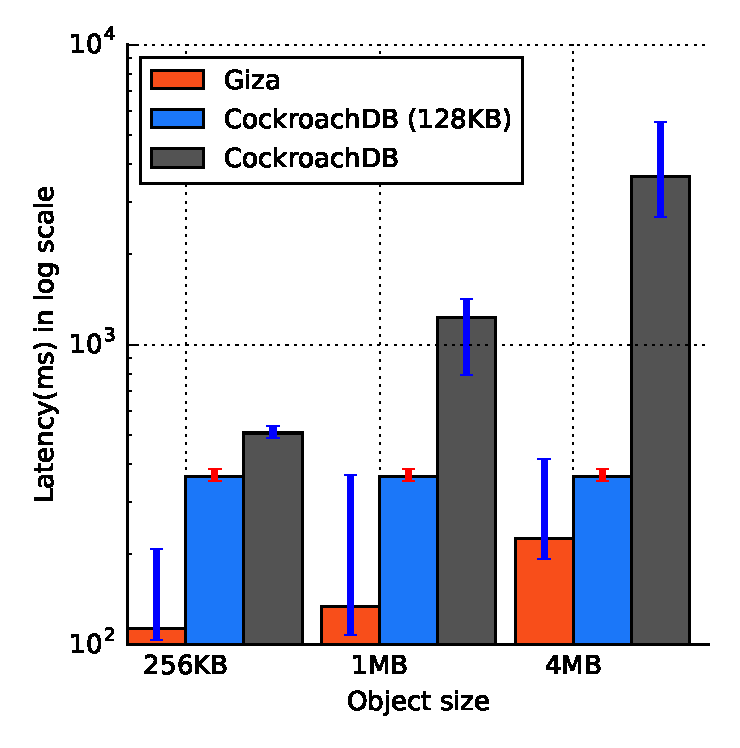
\includegraphics[width=\linewidth]{plots/giza_cock_put}

      % \placeholder{
      %   x-axis: \# clients / partition\\
      %   y-axis: cluster throughput\\
      %   lines: \name{}, OCC, 2PL, TAPIR\\
      %   }
%                \vspace{-1\baselineskip}
      \caption{Put}
      \label{fig:eval_cock_put}
    \end{subfigure}
%    \begin{subfigure}{0.33\textwidth}
%      \includegraphics[width=\linewidth]{figs/graphs/multi_dc/tpcc/tpcc_NEW_ORDER_tpcc_client_lat90.eps}
%
%      % \placeholder{
%      %   x-axis: \# clients / partition\\
%      %   y-axis: latency (median, p90, p99)\\
%      %   (maybe only show median and p99 or just median and report typical distribution)\\
%      %   lines: \name{}, OCC, 2PL, TAPIR\\
%      % }
%      \caption{90\% Latency}
%      \label{fig:geo_tpcc_latency}
%    \end{subfigure}
    \begin{subfigure}{0.45\textwidth}
      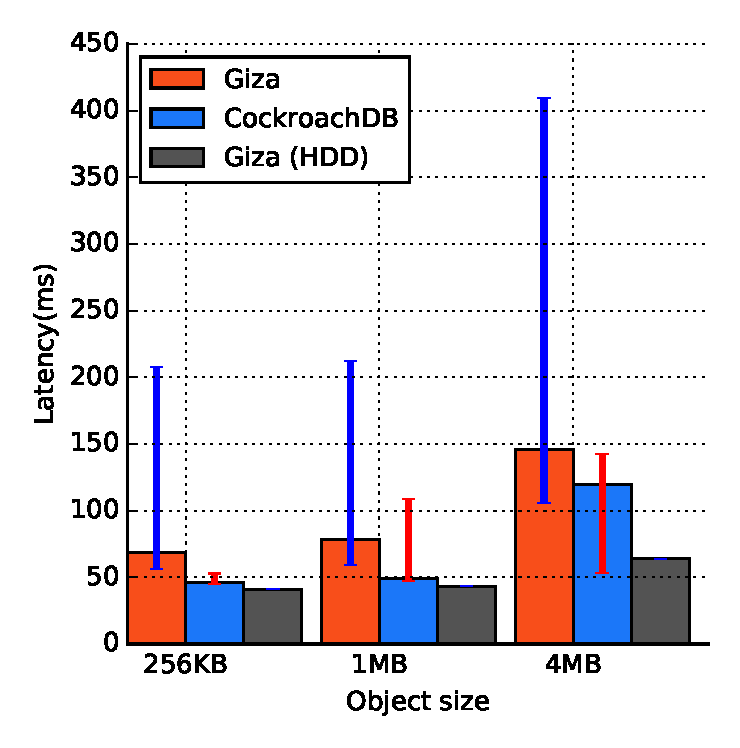
\includegraphics[width=\linewidth]{plots/giza_cock_get}

      % \placeholder{
      %   x-axis: \# clients / partition\\
      %   y-axis: commit rate\\
      %   lines: \name{}, OCC, 2PL, TAPIR\\
      % }
      %\includegraphics[width=\linewidth]{fig/kodiak/tpcc_mix_10_nlog_ct_cr.pdf}
%                \vspace{-1\baselineskip}
      \caption{Get}
      \label{fig:eval_cock_get}
    \end{subfigure}
%  }
  \caption{Performance for \name in different setups}
\end{figure}
% \begin{figure}[t]
% %  \centerline {
%       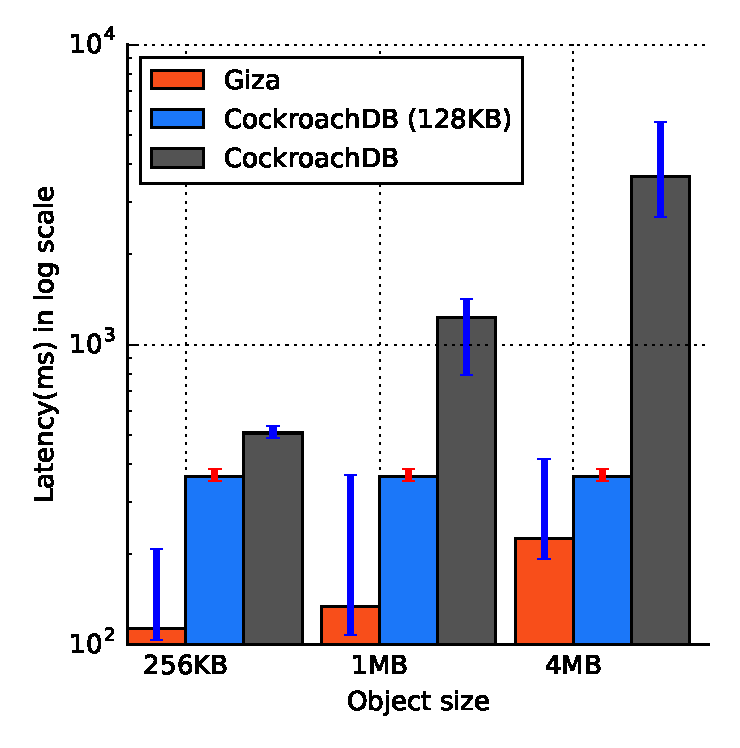
\includegraphics[width=\linewidth]{plots/giza_cock_put}
%       \caption{CockroachDB vs Giza Put with various object sizes}
%       \label{fig:eval_cock_put}
% %  }
% \end{figure}

% %\begin{figure}[t]
% %  \centerline {
% %      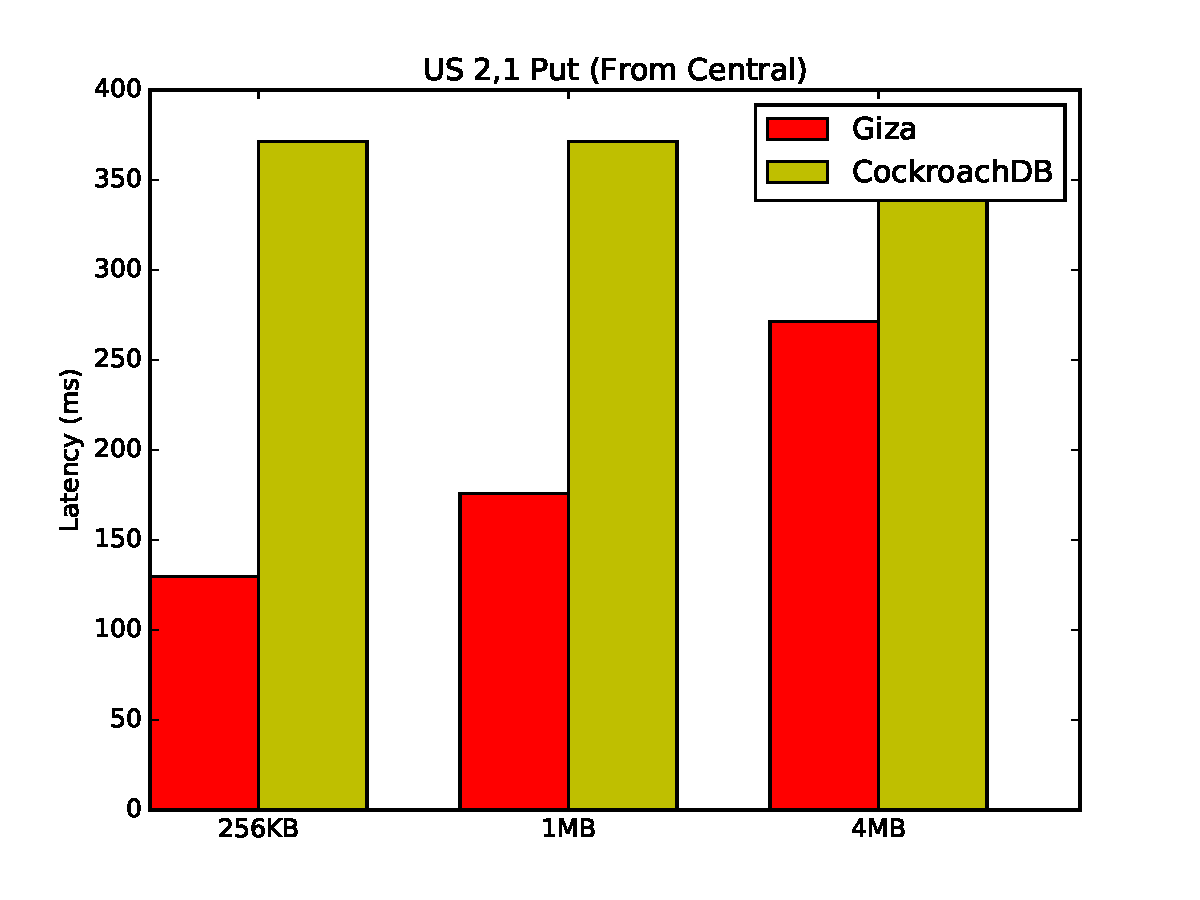
\includegraphics[width=\linewidth]{images/cockroach_vs_giza_put_128}
% %      \caption{CockroachDB vs Giza with various object sizes}
% %      \label{fig:eval_cock_put2}
% %  }
% %\end{figure}

% \begin{figure}[t]
% %  \centerline {
%       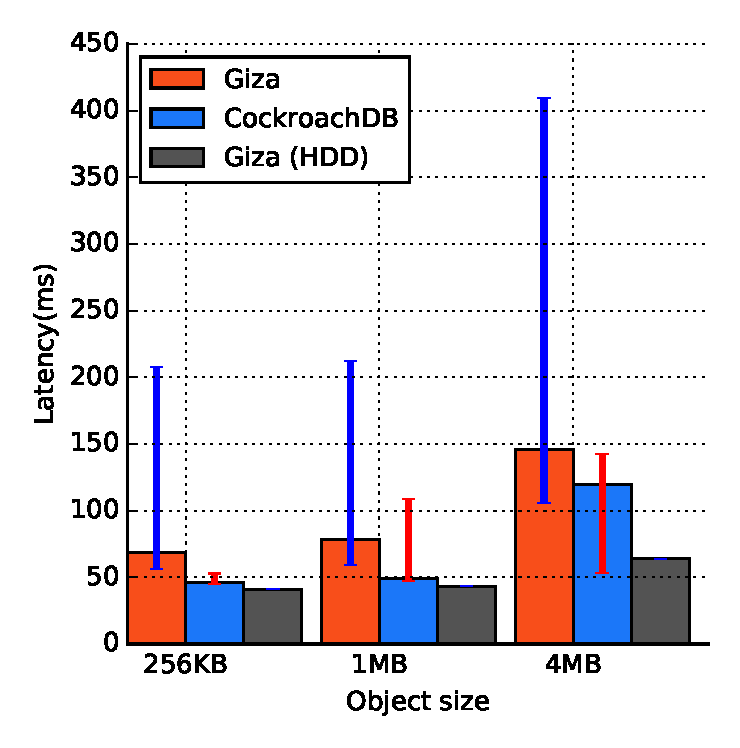
\includegraphics[width=\linewidth]{plots/giza_cock_get}
%       \caption{CockroachDB vs Giza Get with various object sizes}
%       \label{fig:eval_cock_get}
% %  }
% \end{figure}
%%% Local Variables:
%%% mode: latex
%%% TeX-master: "main"
%%% End:


\sm {
  In this section, I will have two graphs. One comparing Giza's full write path with CockroachDB's full replication. Another one is comparing the metadata path with cockroach db. This is to show, hopefully, that the fast paxos scheme is better. I will probably have 3 graphs each making request from one of the three datacenters. Due to multipaxos, there might be extra latency for cockroachdb's case.
}
We benchmark the performance of Giza with CockroachDB in two cases. In the first case, we use CockroachDB as a geo-replicating blah blah blah. Here is the result.
In the second case, we used cockroachdb's transaction to simulate what we are doing with Giza. Blah blah blah, here is the result.
64K $\sim$ 16MB

X-axis: Value size
Y-axis: 50\% Read latency

X-axis: Value size
Y-axis: 90\% Read latency

X-axis: Value size
Y-axis: 99\% Read latency

Same for write

[adding cpu results in a table]

% \subsection{Large object}
% 256MB $\sim$ 1GB

% X-axis: Value size
% Y-axis: Average Read latency

% X-axis: Value size
% Y-axis: Average Write latency


% \subsection{Contention}

% Fixed object size
% X-axis: zipf coefficient
% Y-axis: 50\%, 90\%, 99\% Read/Write Latency


% \subsection{Real workload}
% Table.


%%% Local Variables:
%%% mode: latex
%%% TeX-master: "main"
%%% End:

